\ifdefined\inMainDoc\else
\documentclass[12pt,a4paper]{article}
% ================================================================
%  PRÉAMBULE COMMUN - ANNALES CORRIGÉES
%  Université de Kara - FaST - Licence Fondamentale MPC
%  Design optimisé impression noir et blanc
% ================================================================

% -- ENCODAGE & LANGUE --
\usepackage[utf8]{inputenc}
\usepackage[T1]{fontenc}
\usepackage[french]{babel}
\usepackage{lmodern}
\usepackage{microtype}

% -- MISE EN PAGE --
\usepackage[a4paper, top=2.8cm, bottom=2.5cm, left=2.5cm, right=2.5cm, headheight=14pt]{geometry}
\usepackage{setspace}
\setstretch{1.2}
\usepackage{parskip}
\setlength{\parindent}{1.2em}
\setlength{\parskip}{4pt}

% -- MATHS --
\usepackage{amsmath, amssymb, mathtools, amsthm}
\usepackage{mathrsfs}
\usepackage{dsfont}
\usepackage{bm}
\usepackage{cancel}
\usepackage{textcomp}
% Définition de \oiint (intégrale de surface fermée) sans package supplémentaire
\newcommand{\oiint}{\mathop{\iint\!\!\!\!\!\!\!\bigcirc}\limits}

% -- PHYSIQUE & CHIMIE --
\usepackage{physics}
\usepackage{siunitx}
% Lorsque physics est chargé, siunitx omet \qty. On le restaure ici :
\AtBeginDocument{\RenewCommandCopy\qty\SI}
\sisetup{locale = FR, detect-all, output-decimal-marker={,}}
% Commande de substitution pour les unités posant problème avec pdflatex
% (ohm, degreeCelsius, micro, angstrom, percent utilisent des caractères non-ASCII)
\newcommand{\qtyohm}[1]{\ensuremath{\num{#1}\,\Omega}}
\newcommand{\qtydegc}[1]{\ensuremath{\num{#1}\,{}^\circ\text{C}}}
\newcommand{\qtyangstrom}[1]{\ensuremath{\num{#1}\,\text{\AA}}}
\newcommand{\qtypercent}[1]{\ensuremath{\num{#1}\,\%}}
\newcommand{\qtyum}[1]{\ensuremath{\num{#1}\,\mu\text{m}}}
\usepackage[version=4]{mhchem}

% -- GRAPHISMES --
\usepackage{graphicx}
\usepackage{float}
\usepackage{caption}
\usepackage{subcaption}
\usepackage{wrapfig}
\usepackage{tikz}
\usetikzlibrary{calc, arrows.meta, patterns, shapes.geometric}
\usepackage{pgfplots}
\pgfplotsset{compat=1.18}

% -- TABLEAUX --
\usepackage{booktabs}
\usepackage{array}
\usepackage{tabularx}
\usepackage{multirow}

% -- LISTES --
\usepackage{enumitem}
\setlist[enumerate]{topsep=3pt, itemsep=2pt, parsep=0pt}
\setlist[itemize]{topsep=3pt, itemsep=2pt, parsep=0pt, label={.}}

% -- BOÎTES (noir et blanc) --
\usepackage{mdframed}
\usepackage{tcolorbox}
\tcbuselibrary{skins, breakable, theorems}

% Boîte EXERCICE : encadré avec filet épais, fond blanc
\newmdenv[
  linewidth=1.2pt,
  linecolor=black,
  roundcorner=3pt,
  skipabove=10pt,
  skipbelow=6pt,
  innertopmargin=8pt,
  innerbottommargin=8pt,
  innerleftmargin=10pt,
  innerrightmargin=10pt,
  backgroundcolor=white,
  frametitle={\bfseries\small Exercice},
  frametitlealignment=\raggedright,
  frametitleaboveskip=4pt,
  frametitlebelowskip=4pt,
]{boiteexercice}

% Boîte CORRIGÉ : fond gris très clair + filet fin
\newmdenv[
  linewidth=0.6pt,
  linecolor=black,
  leftline=true,
  rightline=false,
  topline=false,
  bottomline=false,
  linecolor=black,
  innerleftmargin=12pt,
  innerrightmargin=8pt,
  innertopmargin=6pt,
  innerbottommargin=6pt,
  backgroundcolor=gray!8,
  skipabove=4pt,
  skipbelow=8pt,
]{boitecorrige}

% Boîte RÉSUMÉ DE COURS : double encadré
\newmdenv[
  linewidth=0.8pt,
  linecolor=black,
  roundcorner=2pt,
  backgroundcolor=gray!12,
  innertopmargin=10pt,
  innerbottommargin=10pt,
  innerleftmargin=12pt,
  innerrightmargin=12pt,
  skipabove=12pt,
  skipbelow=8pt,
]{boiteresume}

% Boîte ATTENTION/REMARQUE : barre gauche épaisse
\newmdenv[
  leftline=true,
  rightline=false,
  topline=false,
  bottomline=false,
  linewidth=3pt,
  linecolor=black,
  backgroundcolor=gray!5,
  innerleftmargin=12pt,
  innerrightmargin=8pt,
  innertopmargin=5pt,
  innerbottommargin=5pt,
  skipabove=6pt,
  skipbelow=6pt,
]{boiteremarque}

% -- DIFFICULTÉ DES EXERCICES --
\newcommand{\facile}{$\star$}
\newcommand{\moyen}{$\star\!\star$}
\newcommand{\difficile}{$\star\!\star\!\star$}
\newcommand{\niveau}[1]{\hfill\textbf{#1}\hspace{2pt}}

% -- EN-TÊTES ET PIEDS DE PAGE --
\usepackage{fancyhdr}
\pagestyle{fancy}
\fancyhf{}
\renewcommand{\headrulewidth}{0.5pt}
\renewcommand{\footrulewidth}{0.3pt}

% -- HYPERLIENS --
\usepackage[hidelinks]{hyperref}
\hypersetup{
    colorlinks=false,
    pdftitle={Annale Corrigée - Licence MPC - Université de Kara}
}

% -- TITRES --
\usepackage{titlesec}
\titleformat{\section}{\Large\bfseries}{\thesection.}{0.8em}{}[\vspace{2pt}\hrule\vspace{4pt}]
\titleformat{\subsection}{\large\bfseries}{\thesubsection.}{0.7em}{}
\titleformat{\subsubsection}{\normalsize\bfseries}{\thesubsubsection.}{0.6em}{}

% -- THÉORÈMES --
\theoremstyle{definition}
\newtheorem{defn}{Définition}[section]
\newtheorem{prop}{Propriété}[section]
\newtheorem{thm}{Théorème}[section]
\newtheorem{corol}{Corollaire}[section]
\newtheorem{exemple}{Exemple}[section]

% -- COMMANDES MATHÉMATIQUES UTILES --
\newcommand{\vect}[1]{\overrightarrow{#1}}
\newcommand{\R}{\mathbb{R}}
\newcommand{\N}{\mathbb{N}}
\newcommand{\Z}{\mathbb{Z}}
\newcommand{\C}{\mathbb{C}}
\renewcommand{\d}{\mathrm{d}}
\newcommand{\deriv}[2]{\dfrac{\d #1}{\d #2}}
\newcommand{\dpart}[2]{\dfrac{\partial #1}{\partial #2}}
\newcommand{\rot}{\overrightarrow{\mathrm{rot}}\,}
\renewcommand{\div}{\mathrm{div}\,}
\renewcommand{\grad}{\overrightarrow{\mathrm{grad}}\,}
\newcommand{\e}{\mathrm{e}}
\newcommand{\ii}{\mathrm{i}}
\renewcommand{\Tr}{\mathrm{Tr}}

% Numérotation des équations par section
\numberwithin{equation}{section}

% -- RÉSULTATS ENCADRÉS --
\newcommand{\res}[1]{\[\boxed{#1}\]}

% -- REMARQUE INLINE --
\newcommand{\rmq}[1]{\begin{boiteremarque}\textbf{Remarque.} #1\end{boiteremarque}}

% -- MISE EN VALEUR DU RÉSULTAT FINAL --
\newcommand{\reponse}[1]{%
  \begin{center}
    \fbox{\begin{minipage}{0.92\textwidth}\centering #1\end{minipage}}
  \end{center}%
}


% En-têtes spécifiques à ce fichier
\lhead{\small\textit{Atomistique - Licence 1}}
\rhead{\small\textit{FaST, Université de Kara}}
\cfoot{\thepage}

\begin{document}
\fi

\begin{center}
  {\LARGE\bfseries ATOMISTIQUE}\\[0.3cm]
  {\normalsize Licence 1 - Mathématiques, Physique et Chimie}\\[0.1cm]
  \rule{0.7\textwidth}{0.8pt}
\end{center}

\vspace{0.3cm}

% ================================================================
\section*{Résumé du cours}
% ================================================================

\begin{boiteresume}

\textbf{1. Le modèle de Bohr.} L'atome d'hydrogène est formé d'un proton et d'un électron gravitant sur une orbite circulaire de rang $n$ (nombre quantique principal, $n \in \mathbb{N}^*$). Les hypothèses de Bohr imposent la quantification du moment cinétique orbital : $L = m_e v r = n\hbar$, avec $\hbar = h/(2\pi)$.

Le rayon de l'orbite de rang $n$ et l'énergie associée pour un atome hydrogénoïde de numéro atomique $Z$ sont :
\[
r_n = \frac{n^2}{Z}\,a_0 \qquad \text{avec} \qquad a_0 = \frac{\varepsilon_0 h^2}{\pi m_e e^2} \approx \qtyangstrom{0.529}
\]
\[
E_n = -\frac{Z^2}{n^2}\,E_1^{(H)} \qquad \text{avec} \qquad E_1^{(H)} = \qty{-13.6}{eV}
\]

\textbf{2. Configurations électroniques.} Le remplissage des sous-couches obéit à trois règles :
\begin{itemize}[nosep]
  \item \textbf{Règle de Klechkowski} : remplissage dans l'ordre croissant de $n+\ell$, puis par $n$ croissant en cas d'égalité. Ordre pratique : 1s, 2s, 2p, 3s, 3p, 4s, 3d, 4p, 5s, 4d, \dots
  \item \textbf{Règle de Pauli} : deux électrons d'une même case ont nécessairement des spins antiparallèles ; aucune case ne peut contenir plus de deux électrons.
  \item \textbf{Règle de Hund} : à sous-couche partiellement remplie, les électrons occupent d'abord chacun une case différente, avec des spins parallèles.
\end{itemize}

\textbf{3. Orbitales moléculaires (OM).} La combinaison linéaire d'orbitales atomiques (CLOA) donne des OM liantes ($\sigma$, $\pi$) et antiliantes ($\sigma^*$, $\pi^*$). L'ordre de remplissage pour les molécules homodiatomiques de la 2\textsuperscript{e} période est :
$\sigma_{1s} < \sigma^*_{1s} < \sigma_{2s} < \sigma^*_{2s} < (\pi_{2p_x}, \pi_{2p_y}) < \sigma_{2p_z} < \dots$

L'indice de liaison vaut : $\omega = \dfrac{N_l - N_{al}}{2}$, où $N_l$ est le nombre d'électrons liants et $N_{al}$ le nombre d'antiliants.

\textbf{4. Transition énergétique et longueur d'onde.} L'énergie d'un photon émis ou absorbé lors d'une transition $n_i \to n_f$ est :
\[
\Delta E = E_{n_f} - E_{n_i} = h\nu = \frac{hc}{\lambda}
\]
Si $\Delta E < 0$ : émission ; si $\Delta E > 0$ : absorption.

\end{boiteresume}

\newpage

% ================================================================
\section{Modèle de Bohr et atomes hydrogénoïdes}
% ================================================================

\subsection*{Exercice 1 - Isotopes du carbone et masse atomique de l'azote \niveau{\facile}}

\begin{boiteexercice}
Un atome de carbone de masse atomique 12 possède un isotope de masse atomique 14. L'azote naturel est composé de deux isotopes : $^{14}_{7}$N (abondance \qtypercent{99.635}) et $^{15}_{7}$N (abondance \qtypercent{0.365}), de masses atomiques respectives \qty{14.007515}{u} et \qty{15.004863}{u}.

\begin{enumerate}
  \item Définir isotope et donner le nombre de neutrons de chaque isotope du carbone.
  \item Calculer la masse atomique moyenne de l'azote naturel.
\end{enumerate}
\end{boiteexercice}

\begin{boitecorrige}
\textbf{1.} Deux isotopes d'un même élément ont le même numéro atomique $Z$ mais des nombres de masse $A$ différents (donc des nombres de neutrons $N = A - Z$ différents).

Pour le carbone ($Z = 6$) : $^{12}_{6}$C possède $12 - 6 = 6$ neutrons ; $^{14}_{6}$C en possède $14 - 6 = 8$.

\textbf{2.} La masse atomique moyenne de l'azote naturel est la moyenne pondérée par les abondances isotopiques :
\[
\overline{M} = \frac{99{,}635}{100} \times 14{,}007515 + \frac{0{,}365}{100} \times 15{,}004863
\]
\[
\overline{M} = 13{,}9704 + 0{,}0548 \approx \qty{14.01}{g.mol^{-1}}
\]
\end{boitecorrige}

\begin{center}
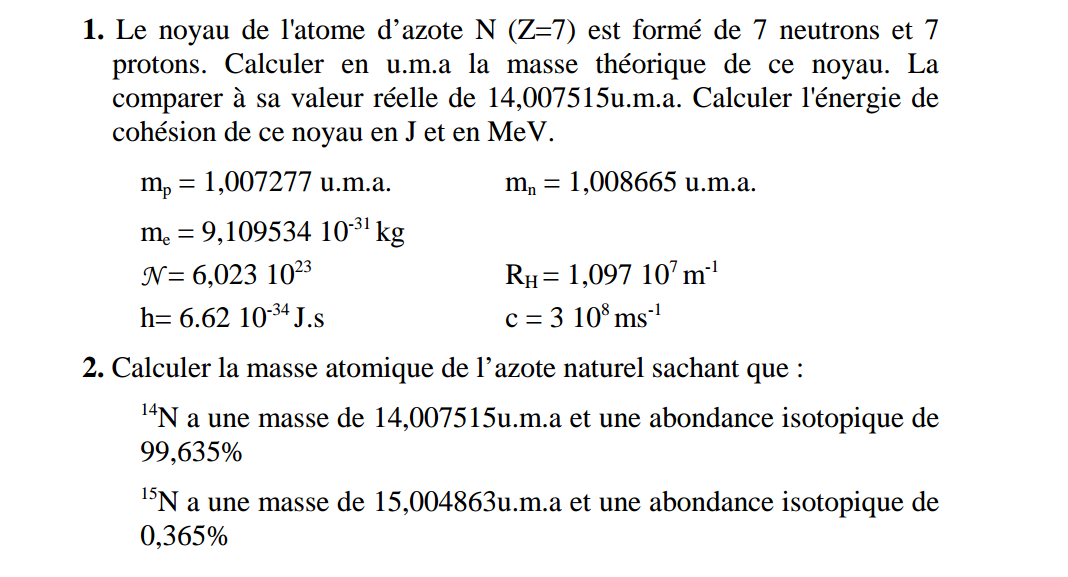
\includegraphics[width=0.6\textwidth]{images/atomistique/atom-001-000.png}
\captionof{figure}{\small Isotopes du carbone : $^{12}_6\text{C}$ et $^{14}_6\text{C}$, même $Z=6$, $A$ différents.}
\end{center}
\begin{center}
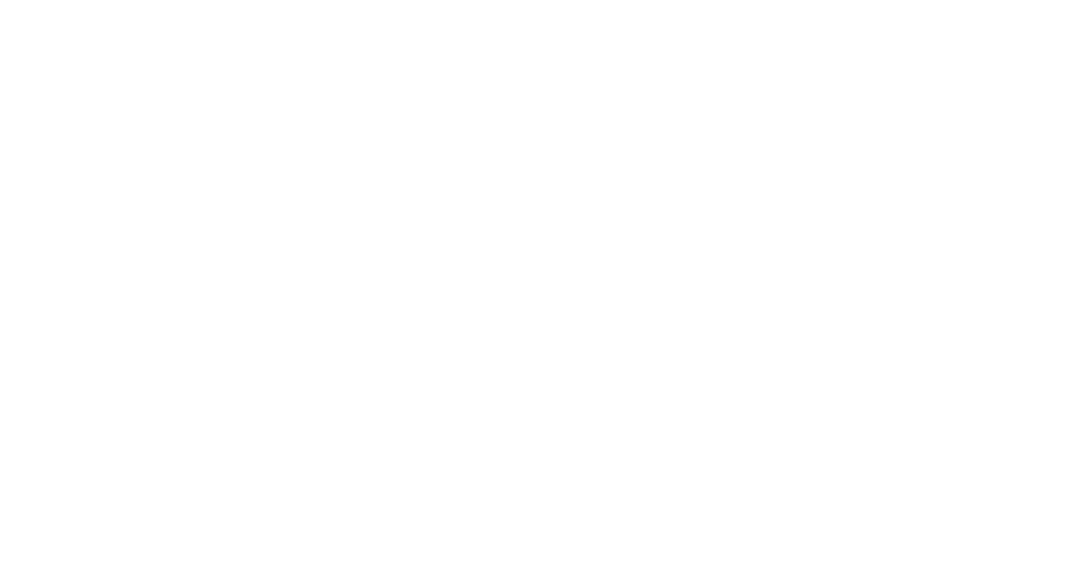
\includegraphics[width=0.6\textwidth]{images/atomistique/atom-001-001.png}
\captionof{figure}{\small Isotopes de l'azote : $^{14}_7\text{N}$ (majoritaire) et $^{15}_7\text{N}$ (trace).}
\end{center}
\begin{center}
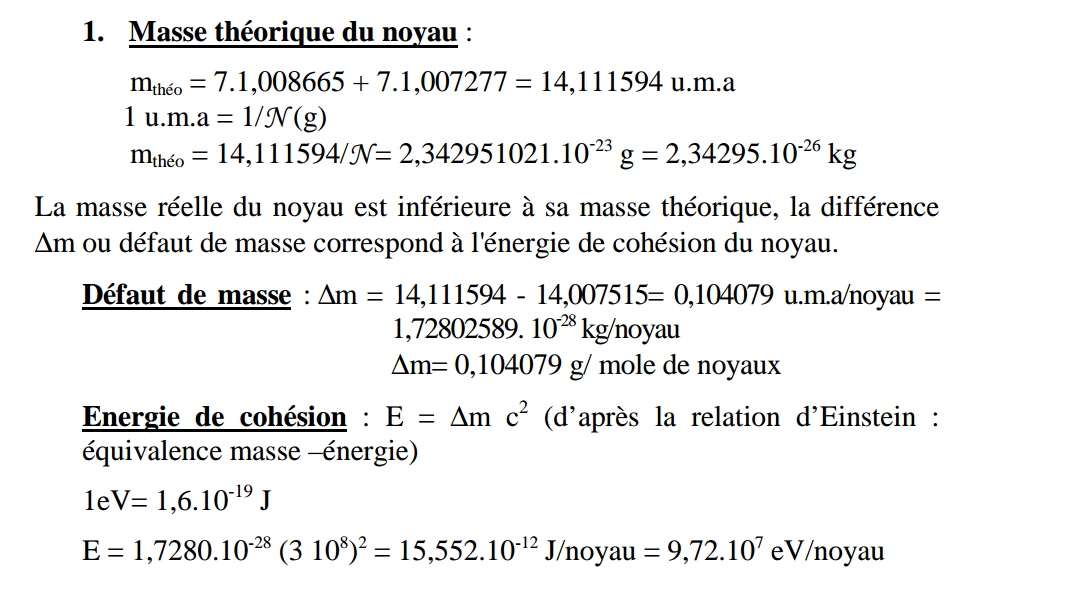
\includegraphics[width=0.6\textwidth]{images/atomistique/atom-001-002.png}
\captionof{figure}{\small Composition du noyau : protons et neutrons des isotopes de l'azote.}
\end{center}
\begin{center}
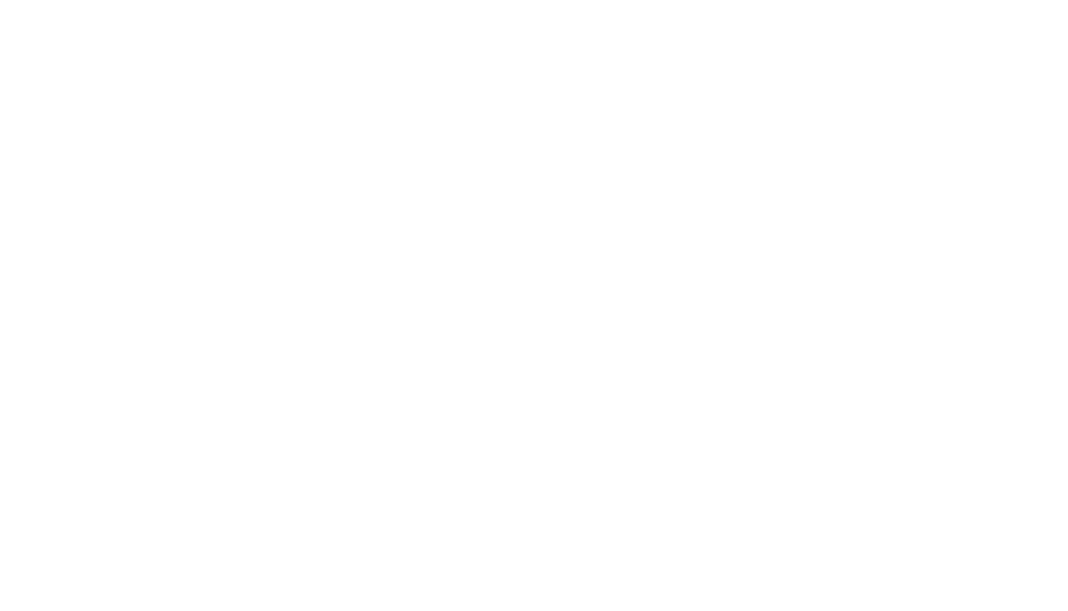
\includegraphics[width=0.6\textwidth]{images/atomistique/atom-001-003.png}
\captionof{figure}{\small Calcul de la masse atomique moyenne par pondération des abondances.}
\end{center}

\subsection*{Exercice 2 - Atome hydrogénoïde : modèle de Bohr \niveau{\moyen}}

\begin{boiteexercice}
Pour un atome hydrogénoïde (noyau de charge $+Ze$ autour duquel gravite un électron) :

\begin{enumerate}
  \item Établir les formules donnant :
    \begin{enumerate}[label=(\alph*)]
      \item le rayon $r_n$ de l'orbite de rang $n$,
      \item l'énergie totale $E_n$ du système noyau-électron,
      \item les expressions de $r_n$ et $E_n$ en fonction des grandeurs correspondantes de l'hydrogène.
    \end{enumerate}
  \item Calculer en eV et en joules les énergies des quatre premiers niveaux de l'ion $\text{Li}^{2+}$.
  \item Quelle énergie doit absorber un ion $\text{Li}^{2+}$ pour que l'électron passe du niveau fondamental au premier niveau excité ?
  \item Si cette énergie est fournie sous forme lumineuse, calculer la longueur d'onde $\lambda$ du rayonnement correspondant.
\end{enumerate}

\textbf{Données :} $\text{Li}(Z=3)$, $1\,\text{eV} = \qty{1.6e-19}{J}$, $c = \qty{3e8}{m.s^{-1}}$, $h = \qty{6.62e-34}{J.s}$.
\end{boiteexercice}

\begin{boitecorrige}
\textbf{1.(a) Rayon de l'orbite.}

L'électron est en équilibre entre la force électrostatique et la force centrifuge :
\[
\frac{Ze^2}{4\pi\varepsilon_0 r^2} = \frac{m_e v^2}{r} \tag{1}
\]
La quantification de Bohr impose $m_e v r = n\hbar$, soit :
\[
v = \frac{n\hbar}{m_e r} \tag{2}
\]
En substituant (2) dans (1) :
\[
\boxed{r_n = \frac{n^2}{Z}\cdot\frac{\varepsilon_0 h^2}{\pi m_e e^2} = \frac{n^2}{Z}\,a_0}
\]

\textbf{1.(b) Énergie totale.}

L'énergie cinétique $E_c = \frac{1}{2}m_e v^2$ et l'énergie potentielle $E_p = -\frac{Ze^2}{4\pi\varepsilon_0 r}$. La condition d'équilibre (1) donne $E_c = -\frac{1}{2}E_p$, d'où $E_t = E_c + E_p = \frac{1}{2}E_p$ :
\[
\boxed{E_n = -\frac{Z^2}{n^2}\cdot\frac{m_e e^4}{8\varepsilon_0^2 h^2} = -\frac{Z^2}{n^2}\,E_1^{(H)}}
\]

\textbf{1.(c) Expressions relatives à l'hydrogène.}

Pour $Z=1$, $n=1$ : $a_0 = (r_1)_H \approx \qtyangstrom{0.529}$ et $E_1^{(H)} = -\qty{13.6}{eV}$. Ainsi :
\[
r_n = \frac{n^2}{Z}\,(r_1)_H \qquad \text{et} \qquad E_n = -\frac{Z^2}{n^2}\times\qty{13.6}{eV}
\]

\textbf{2. Niveaux d'énergie de Li$^{2+}$ ($Z=3$).}

$(E_1)_{\text{Li}^{2+}} = -Z^2 \times \qty{13.6}{eV} = -9 \times \qty{13.6}{eV} = \qty{-122.4}{eV}$

\begin{center}
\begin{tabular}{ccc}
\toprule
$n$ & $E_n$ (eV) & $E_n$ (J) \\
\midrule
1 & $-122{,}4$ & $\qty{-1.96e-17}{}$ \\
2 & $-30{,}6$ & $\qty{-4.90e-18}{}$ \\
3 & $-13{,}6$ & $\qty{-2.18e-18}{}$ \\
4 & $-7{,}65$ & $\qty{-1.22e-18}{}$ \\
\bottomrule
\end{tabular}
\end{center}

\textbf{3. Énergie à absorber pour la transition $n=1 \to n=2$.}

\[
\Delta E = E_2 - E_1 = -30{,}6 - (-122{,}4) = \qty{91.8}{eV} = \qty{1.47e-17}{J}
\]

\textbf{4. Longueur d'onde correspondante.}

\[
\lambda = \frac{hc}{\Delta E} = \frac{6{,}62\times10^{-34}\times3\times10^8}{1{,}47\times10^{-17}} \approx \qty{13.5}{nm}
\]
Ce rayonnement est dans le domaine ultraviolet lointain.
\end{boitecorrige}

\begin{center}
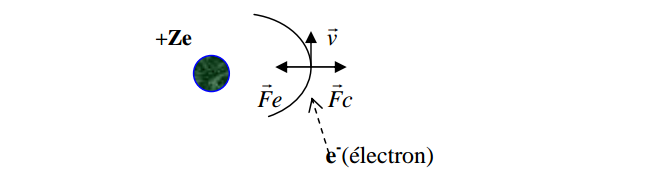
\includegraphics[width=0.55\textwidth]{images/atomistique/atom-002-004.png}
\captionof{figure}{\small Modèle de Bohr de l'atome d'hydrogène : orbites circulaires quantifiées de rayon $r_n = n^2 a_0/Z$.}
\end{center}
\begin{center}
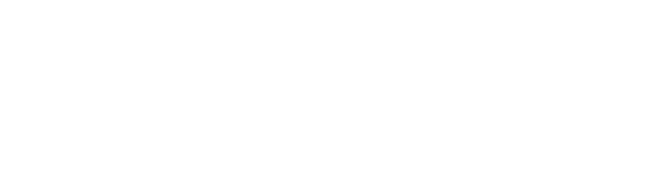
\includegraphics[width=0.55\textwidth]{images/atomistique/atom-002-005.png}
\captionof{figure}{\small Niveaux d'énergie $E_n = -Z^2 E_1^{(H)}/n^2$ de l'ion hydrogénoïde $\text{Li}^{2+}$ ($Z=3$).}
\end{center}

\subsection*{Exercice 3 - Transitions énergétiques de l'atome d'hydrogène \niveau{\moyen}}

\begin{boiteexercice}
\begin{enumerate}
  \item Un atome d'hydrogène initialement à l'état fondamental absorbe \qty{10.2}{eV}. À quel niveau se retrouve l'électron ?
  \item L'électron d'un atome d'hydrogène initialement au niveau $n=3$ émet un rayonnement de longueur d'onde $\lambda = \qtyangstrom{1027}$. À quel niveau se retrouve l'électron ?
\end{enumerate}
\end{boiteexercice}

\begin{boitecorrige}
\textbf{1.} L'énergie absorbée depuis l'état fondamental ($n_i = 1$) est :
\[
\Delta E = E_{n_f} - E_1 = \qty{-13.6}{eV}\left(\frac{1}{n_f^2} - 1\right) = \qty{10.2}{eV}
\]
\[
\frac{1}{n_f^2} = 1 - \frac{10{,}2}{13{,}6} = 0{,}25 \quad \Rightarrow \quad n_f = 2
\]
L'électron se retrouve au niveau $n = 2$.

\textbf{2.} L'énergie emportée par le photon émis est :
\[
|\Delta E| = \frac{hc}{\lambda} = \frac{6{,}62\times10^{-34}\times3\times10^8}{1027\times10^{-10}} = \qty{1.934e-18}{J} = \qty{12.09}{eV}
\]
Depuis $n_i = 3$ :
\[
\Delta E = E_{n_f} - E_3 = \qty{-13.6}{eV}\left(\frac{1}{n_f^2} - \frac{1}{9}\right) = -\qty{12.09}{eV}
\]
\[
\frac{1}{n_f^2} = \frac{1}{9} - \frac{12{,}09}{13{,}6} \approx \frac{1}{9} - 0{,}889 \approx -0{,}778
\]

Cela ne donne pas de solution positive. Revoyons le calcul : l'émission signifie $E_{n_f} < E_{n_i} = E_3 = \qty{-1.51}{eV}$. La condition est :
\[
\frac{1}{n_f^2} - \frac{1}{9} = \frac{|\Delta E|}{13{,}6} \approx 0{,}889
\]
\[
\frac{1}{n_f^2} = \frac{1}{9} + \frac{12{,}09}{13{,}6} = 0{,}111 + 0{,}889 = 1 \quad \Rightarrow \quad n_f = 1
\]
L'électron retombe au niveau fondamental ($n = 1$).
\end{boitecorrige}

\subsection*{Exercice 4 - Niveaux d'énergie et transitions de l'hydrogène \niveau{\moyen}}

\begin{boiteexercice}
Les niveaux d'énergie de l'atome d'hydrogène sont donnés par $E_n = -\dfrac{13{,}6}{n^2}$ (en eV).

\begin{enumerate}
  \item Calculer les énergies des 4 premiers niveaux.
  \item Quel est le niveau fondamental ?
  \item Considérer la transition $n=3 \to n=2$.
    \begin{enumerate}[label=(\alph*)]
      \item S'agit-il d'une émission ou d'une absorption ?
      \item Calculer la longueur d'onde correspondante.
      \item À quel domaine appartient ce rayonnement ?
    \end{enumerate}
  \item L'atome absorbe un photon de $\lambda = \qty{121.7}{nm}$. Quelle transition entraîne cette absorption ?
\end{enumerate}

\textbf{Données :} $h = \qty{6.62e-34}{J.s}$, $c = \qty{3.00e8}{m.s^{-1}}$, $\qty{1}{eV} = \qty{1.60e-19}{J}$.
\end{boiteexercice}

\begin{boitecorrige}
\textbf{1.} $E_1 = \qty{-13.6}{eV}$, $E_2 = \qty{-3.40}{eV}$, $E_3 = \qty{-1.51}{eV}$, $E_4 = \qty{-0.85}{eV}$.

\textbf{2.} Le niveau fondamental est $E_1 = \qty{-13.6}{eV}$ (niveau le plus bas, $n=1$).

\textbf{3.(a)} La transition $n=3 \to n=2$ correspond à $\Delta E = E_2 - E_3 = -3{,}40 - (-1{,}51) = \qty{-1.89}{eV}$. Comme $\Delta E < 0$, il s'agit d'une \textbf{émission}.

\textbf{3.(b)}
\[
|\Delta E| = \qty{1.89}{eV} = 1{,}89 \times 1{,}60\times10^{-19} = \qty{3.02e-19}{J}
\]
\[
\lambda = \frac{hc}{|\Delta E|} = \frac{6{,}62\times10^{-34}\times3{,}00\times10^8}{3{,}02\times10^{-19}} \approx \qty{657}{nm}
\]

\textbf{3.(c)} $\lambda \approx \qty{657}{nm}$ : rayonnement \textbf{rouge} du domaine visible (raie $H_\alpha$ de la série de Balmer).

\textbf{4.} Énergie du photon absorbé :
\[
\Delta E = \frac{hc}{\lambda} = \frac{6{,}62\times10^{-34}\times3{,}00\times10^8}{121{,}7\times10^{-9}} = \qty{1.63e-18}{J} = \qty{10.2}{eV}
\]
La seule transition qui correspond est $n=1 \to n=2$ : $\Delta E = E_2 - E_1 = -3{,}40 + 13{,}6 = \qty{10.2}{eV}$. \\
L'électron passe du niveau fondamental ($n=1$) au premier niveau excité ($n=2$). C'est la raie $\text{Ly}_\alpha$ de la série de Lyman (UV).
\end{boitecorrige}

\begin{center}
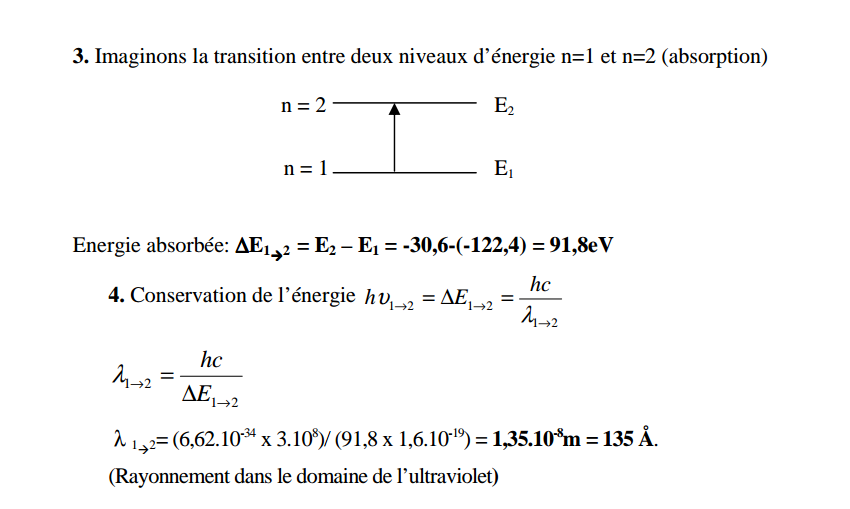
\includegraphics[width=0.55\textwidth]{images/atomistique/atom-004-006.png}
\captionof{figure}{\small Transitions électroniques entre niveaux de Bohr et séries spectrales de l'hydrogène.}
\end{center}
\begin{center}
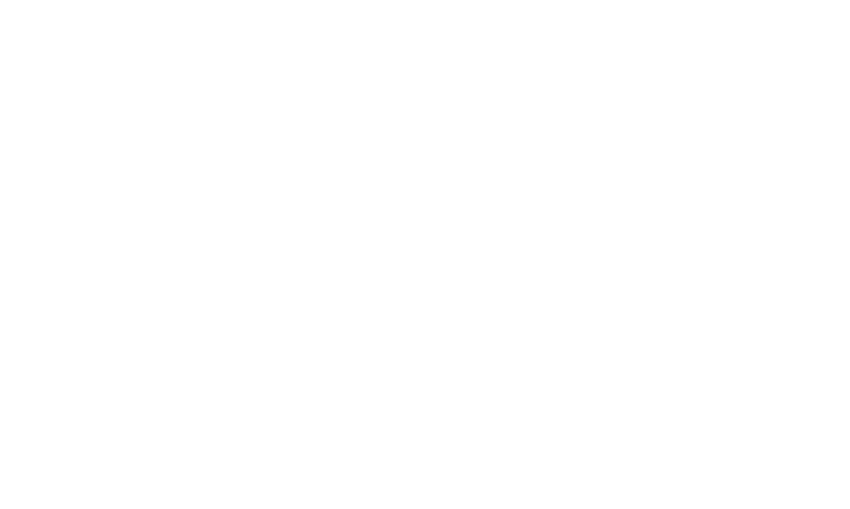
\includegraphics[width=0.55\textwidth]{images/atomistique/atom-004-007.png}
\captionof{figure}{\small Diagramme des séries de Lyman, Balmer et Paschen dans le spectre de l'hydrogène.}
\end{center}

% ================================================================
\section{Structures électroniques et tableau périodique}
% ================================================================

\subsection*{Exercice 5 - Règles de remplissage des structures électroniques \niveau{\facile}}

\begin{boiteexercice}
Parmi les structures électroniques représentées ci-dessous (voir figure), identifier celles qui ne respectent pas les règles de remplissage et expliquer la règle violée.

\begin{center}
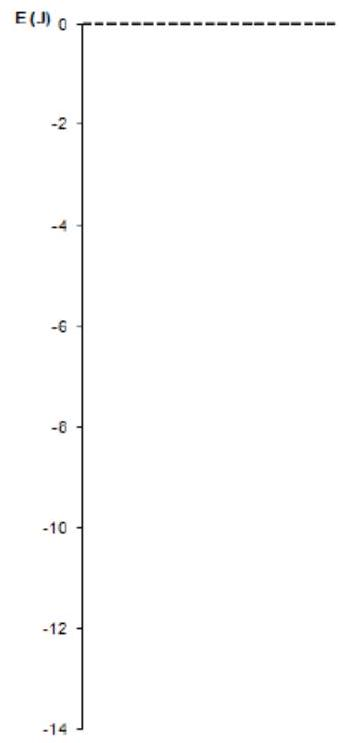
\includegraphics[height=0.55\textheight]{images/atomistique/atom-005-008.png}
\end{center}
\end{boiteexercice}

\begin{boitecorrige}
\begin{itemize}
  \item[(a)] Orbitale $s$ : deux électrons à spins parallèles dans la même case. Violation de la \textbf{règle de Pauli} (deux électrons d'une même case doivent avoir des spins antiparallèles).
  \item[(c)] Orbitale $s$ remplie avant une orbitale de niveau inférieur : violation de la \textbf{règle de Klechkowski} (remplissage dans le mauvais ordre d'énergie).
  \item[(d)] Orbitale $p$ : la première case est vide alors que la deuxième est remplie. Violation de la \textbf{règle de Hund} (il faut distribuer les électrons dans le maximum de cases avant d'en remplir une).
  \item[(e)] Remplissage des sous-couches dans un ordre non conforme à Klechkowski : violation de la \textbf{règle de Klechkowski}.
  \item[(f)] Sous-couche $d$ : des électrons sont appariés avant que toutes les cases soient singly occupied. Violation de la \textbf{règle de Hund}.
\end{itemize}
\end{boitecorrige}

\subsection*{Exercice 6 - Configurations électroniques : N, P et As \niveau{\difficile}}

\begin{boiteexercice}
On considère les éléments $\text{N}_{7}$, $\text{P}_{15}$ et $\text{As}_{33}$.

\begin{enumerate}
  \item Établir leurs configurations électroniques.
  \item Préciser leur position dans le tableau périodique.
  \item Comparer leur électronégativité $\chi$.
  \item Expliquer pourquoi la réaction du chlore avec le phosphore peut conduire à $\text{PCl}_3$ et $\text{PCl}_5$, alors qu'avec l'azote seul $\text{NCl}_3$ se forme. (On note que le chlore est plus électronégatif que l'azote.)
  \item (a) Donner la structure de Lewis de $\text{NH}_3$, $\text{PH}_3$ et $\text{AsH}_3$, et prévoir leur géométrie. (b) Comparer leurs angles de liaison.
  \item Donner la configuration électronique des espèces PN et PN$^+$ et en déduire leurs propriétés magnétiques et le type de liaison.
\end{enumerate}
\end{boiteexercice}

\begin{boitecorrige}
\textbf{1. Configurations électroniques :}
\[
\text{N}_{7} : 1s^{2}\,2s^{2}\,2p^{3} \qquad \text{P}_{15} : 1s^{2}\,2s^{2}\,2p^{6}\,3s^{2}\,3p^{3} \qquad \text{As}_{33} : [\text{Ar}]\,4s^{2}\,3d^{10}\,4p^{3}
\]

\textbf{2. Position dans le tableau :} Ces trois éléments appartiennent à la colonne VA (groupe 15), respectivement aux périodes 2, 3 et 4.

\textbf{3. Électronégativité :} Sur une même colonne, l'électronégativité diminue de haut en bas car le rayon atomique augmente (l'attraction sur les électrons liants est plus faible). Ainsi : $\chi_N > \chi_P > \chi_{As}$.

\textbf{4.} Le phosphore appartient à la troisième période et possède des orbitales $3d$ vides accessibles. Par promotion électronique, il peut porter 5 électrons de valence dans les liaisons, ce qui permet la formation de $\text{PCl}_5$. L'azote, appartenant à la deuxième période, \textbf{ne dispose d'aucune orbitale $d$}. Il ne peut donc pas dépasser la valence 3 (octet strict). La formation de $\text{NCl}_5$ est impossible.

\textbf{5.(a)} Les trois molécules $\text{NH}_3$, $\text{PH}_3$ et $\text{AsH}_3$ ont une géométrie \textbf{pyramidale trigonale} (ou tétraèdre irrégulier) car l'atome central possède un doublet non liant. La structure de Lewis de $\text{NH}_3$ : N avec un doublet libre et trois liaisons N--H.

\textbf{5.(b)} L'angle de liaison $\widehat{\text{HXH}}$ est d'autant plus grand que l'atome central X est électronégatif, car il attire fortement les doublets liants, ce qui accroît la répulsion entre les liaisons. On a donc : $\widehat{\text{HNH}} > \widehat{\text{HPH}} > \widehat{\text{HAsH}}$ (valeurs expérimentales : $107{,}8^\circ $, $93{,}3^\circ $, $91{,}8^\circ $).

\textbf{6.} La molécule PN possède $5 + 5 = 10$ électrons de valence, distribués dans 10 orbitales moléculaires.

Configuration OM de PN (analogie N$_2$) :
\[
\sigma_{2s}^{2}\,\sigma^{*2}_{2s}\,(\pi_{2p_x},\pi_{2p_y})^{4}\,\sigma_{2p_z}^{2}
\]
Tous les électrons sont appariés : PN est \textbf{diamagnétique}. L'indice de liaison $\omega = \frac{(2+4+2)-(2)}{2} = \frac{6}{2} = 3$ : triple liaison (une $\sigma$ et deux $\pi$).

Pour PN$^+$, on retire un électron liant de $\sigma_{2p_z}$ :
\[
\sigma_{2s}^{2}\,\sigma^{*2}_{2s}\,(\pi_{2p_x},\pi_{2p_y})^{4}\,\sigma_{2p_z}^{1}
\]
Un électron célibataire : PN$^+$ est \textbf{paramagnétique}. Indice de liaison $\omega' = 2{,}5$.
\end{boitecorrige}

\begin{center}
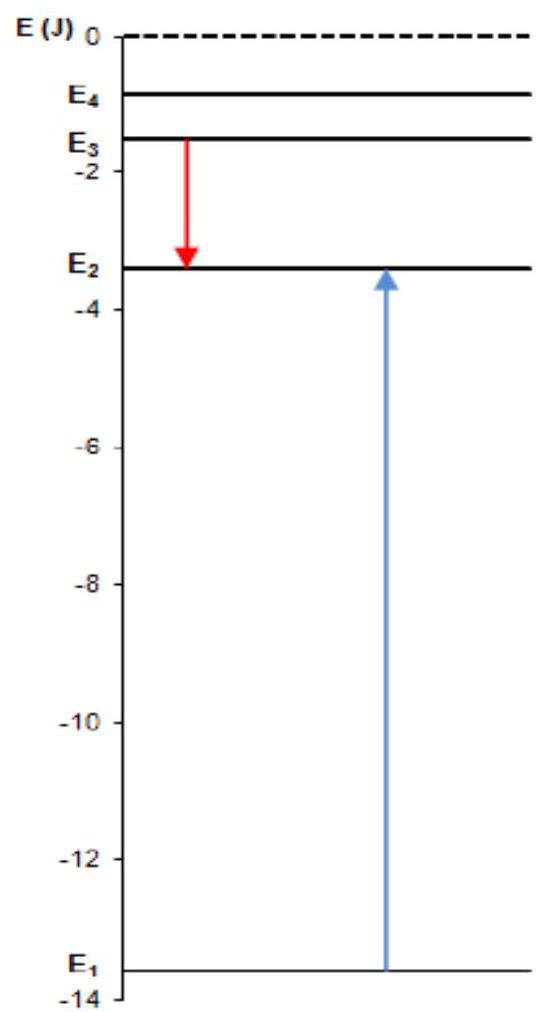
\includegraphics[height=0.55\textheight]{images/atomistique/atom-006-009.png}
\captionof{figure}{\small Diagramme d'énergie des orbitales moléculaires de la molécule PN.}
\end{center}
\begin{center}
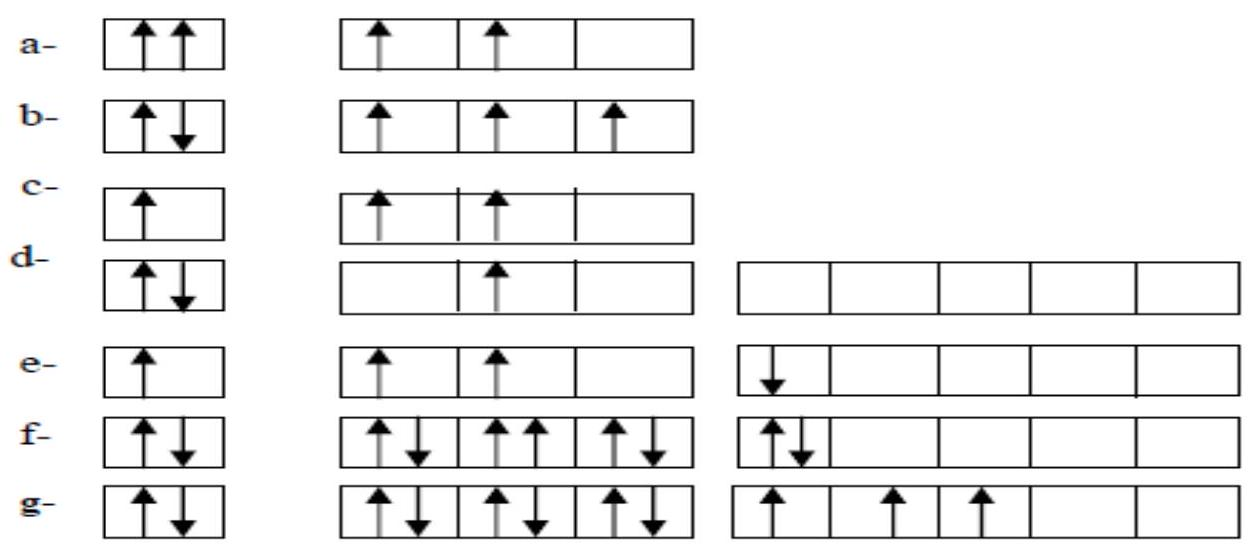
\includegraphics[width=0.55\textwidth]{images/atomistique/atom-006-010.png}
\captionof{figure}{\small Structure de Lewis et géométrie des molécules $\text{NH}_3$, $\text{PH}_3$ et $\text{AsH}_3$.}
\end{center}

\subsection*{Exercice 7 - Identification d'éléments chimiques \niveau{\moyen}}

\begin{boiteexercice}
Donner le numéro atomique et la configuration électronique des éléments suivants :
\begin{enumerate}[label=(\alph*)]
  \item L'halogène de numéro atomique inférieur à 18.
  \item Le gaz rare de même période que le chlore ($Z=17$).
  \item Le troisième halogène.
  \item Le deuxième métal de transition.
  \item Les trois premiers éléments des alcalino-terreux.
\end{enumerate}
\end{boiteexercice}

\begin{boitecorrige}
\begin{enumerate}[label=(\alph*)]
  \item L'halogène de $Z < 18$ : \textbf{Cl}, $Z = 17$ : $[\text{Ne}]\,3s^2\,3p^5$.
  \item Le gaz rare de même période que Cl (période 3) : \textbf{Ar}, $Z = 18$ : $[\text{Ne}]\,3s^2\,3p^6$.
  \item Les halogènes dans l'ordre sont F, Cl, Br... Le troisième est \textbf{Br}, $Z = 35$ : $[\text{Ar}]\,4s^2\,3d^{10}\,4p^5$.
  \item Les métaux de transition commencent en période 4 par Sc ($Z=21$) puis \textbf{Ti} ($Z=22$). Le deuxième métal de transition est donc \textbf{Ti}, $Z = 22$ : $[\text{Ar}]\,4s^2\,3d^2$.
  \item Les alcalino-terreux (groupe 2) : \textbf{Be} ($Z=4$), \textbf{Mg} ($Z=12$), \textbf{Ca} ($Z=20$).
\end{enumerate}
\end{boitecorrige}

\begin{center}
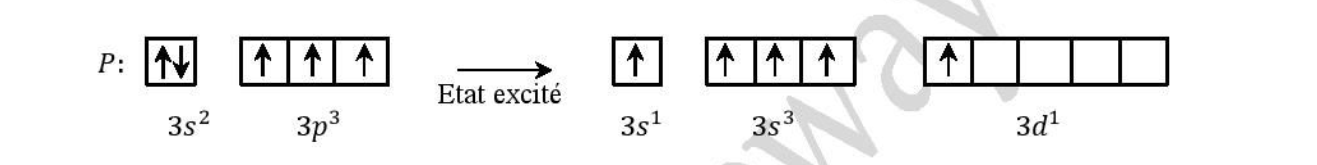
\includegraphics[width=0.55\textwidth]{images/atomistique/atom-007-011.png}
\captionof{figure}{\small Configuration électronique et règle de Klechkowski pour les éléments de transition.}
\end{center}
\begin{center}
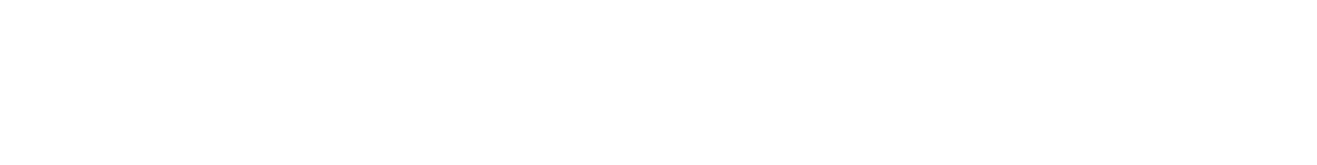
\includegraphics[width=0.55\textwidth]{images/atomistique/atom-007-012.png}
\captionof{figure}{\small Tableau périodique : évolution du rayon atomique et de l'électronégativité.}
\end{center}

\subsection*{Exercice 8 - Configurations électroniques des ions X, Y et Z \niveau{\moyen}}

\begin{boiteexercice}
Donner les configurations électroniques des éléments X, Y et Z sachant que :
\begin{enumerate}[label=(\alph*)]
  \item $X^{3+}$ possède la configuration du Néon ($Z_{\text{Ne}}=10$).
  \item Y appartient à la même période que X, et il lui manque deux électrons pour avoir la configuration d'un gaz rare.
  \item $Z^+$ possède la configuration du gaz rare de la même période que Y.
\end{enumerate}
\end{boiteexercice}

\begin{boitecorrige}
\textbf{(a)} Si $X^{3+}$ a la configuration de Ne (10 électrons), alors X possède $10 + 3 = 13$ électrons. C'est l'Aluminium (Al, $Z = 13$) :
\[
_{13}\text{Al} : [\text{Ne}]\,3s^2\,3p^1
\]

\textbf{(b)} X est en période 3 (puisque $Z=13$). Y est dans la même période, et il lui manque 2 électrons pour atteindre la configuration d'Ar ($Z=18$). Donc Y a $18 - 2 = 16$ électrons : c'est le Soufre (S, $Z=16$) :
\[
_{16}\text{S} : [\text{Ne}]\,3s^2\,3p^4
\]

\textbf{(c)} Y est en période 3, le gaz rare de cette période est Ar ($Z=18$). Si $Z^+$ a la configuration d'Ar (18 électrons), alors Z possède $18 + 1 = 19$ électrons : c'est le Potassium (K, $Z=19$) :
\[
_{19}\text{K} : [\text{Ar}]\,4s^1
\]
\end{boitecorrige}

\begin{center}
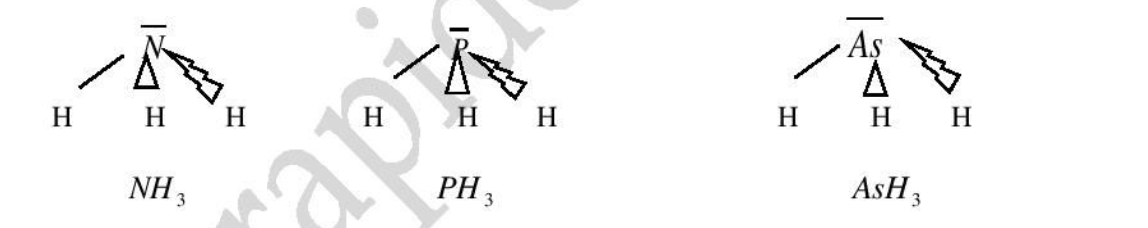
\includegraphics[width=0.55\textwidth]{images/atomistique/atom-008-013.png}
\captionof{figure}{\small Diagramme énergétique des orbitales moléculaires de $\text{O}_2$ : configuration $\sigma$ et $\pi$.}
\end{center}
\begin{center}
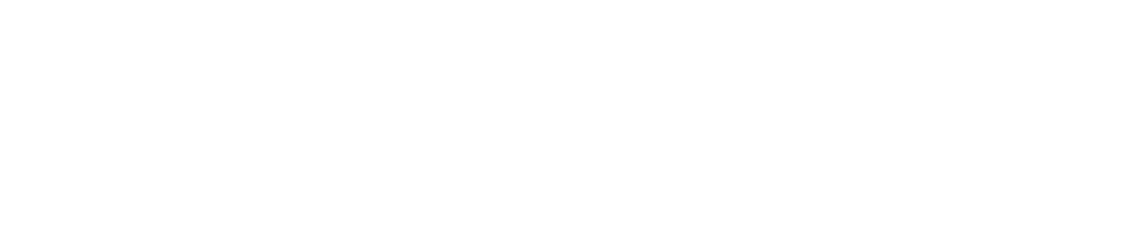
\includegraphics[width=0.55\textwidth]{images/atomistique/atom-008-014.png}
\captionof{figure}{\small Structure de Lewis et géométrie des molécules du second exercice.}
\end{center}

% ================================================================
\section{Liaisons chimiques et orbitales moléculaires}
% ================================================================

\subsection*{Exercice 9 - Énergie d'ionisation et affinité électronique \niveau{\moyen}}

\begin{boiteexercice}
L'énergie d'ionisation (EI) est l'énergie nécessaire pour arracher un électron à un atome à l'état gazeux. L'affinité électronique (AE) est l'énergie libérée lors de la capture d'un électron.
\begin{enumerate}
  \item Donner la configuration électronique de Na ($Z=11$), Mg ($Z=12$), Al ($Z=13$) et Si ($Z=14$).
  \item Expliquer pourquoi l'EI de Mg est supérieure à celle de Na, et pourquoi l'EI d'Al est inférieure à celle de Mg.
  \item Comparer les rayons atomiques de Na, Mg, Al et Si. Expliquer la tendance générale.
  \item L'ion $\text{Na}^+$ et l'atome Ne ont-ils la même configuration électronique ? Comparer leurs rayons.
\end{enumerate}
\end{boiteexercice}

\begin{boitecorrige}
\textbf{1. Configurations électroniques :}
\[
\text{Na} : [\text{Ne}]\,3s^1 \qquad \text{Mg} : [\text{Ne}]\,3s^2 \qquad \text{Al} : [\text{Ne}]\,3s^2\,3p^1 \qquad \text{Si} : [\text{Ne}]\,3s^2\,3p^2
\]

\textbf{2.} Mg possède la sous-couche $3s^2$ entièrement remplie, ce qui confère une stabilité particulière (paire d'électrons appariés). Il faut donc plus d'énergie pour ioniser Mg que Na. L'EI de Mg est supérieure à celle de Na.

Cependant, Al a un électron $3p^1$ qui est légèrement plus haut en énergie et plus éloigné du noyau que les électrons $3s^2$ de Mg. Cet électron $3p$ est aussi moins bien blindé. Résultat : l'EI d'Al est \textit{inférieure} à celle de Mg, malgré $Z$ plus grand.

\textbf{3.} Sur une même période, en allant de gauche à droite, le numéro atomique $Z$ augmente, donc l'attraction nucléaire sur les électrons de valence est plus forte. Le rayon atomique \textbf{diminue} : $r_{\text{Na}} > r_{\text{Mg}} > r_{\text{Al}} > r_{\text{Si}}$.

\textbf{4.} $\text{Na}^+$ a perdu un électron : $[\text{Ne}]\,3s^0 \equiv [\text{Ne}]$. Oui, $\text{Na}^+$ et Ne ont la même configuration à 10 électrons. Cependant, Na$^+$ a $Z=11$ contre $Z=10$ pour Ne : l'attraction nucléaire plus forte de Na$^+$ contracte davantage le nuage électronique. Donc $r_{\text{Na}^+} < r_{\text{Ne}}$.
\end{boitecorrige}

\subsection*{Exercice 10 - Orbitales moléculaires de $\text{O}_2$ \niveau{\difficile}}

\begin{boiteexercice}
La molécule $\text{O}_2$ ($Z_O = 8$) est formée de deux atomes d'oxygène.
\begin{enumerate}
  \item Rappeler la configuration électronique de l'atome O.
  \item Écrire la configuration électronique de $\text{O}_2$ dans le cadre de la théorie des orbitales moléculaires (OM). L'ordre des OM pour $\text{O}_2$ est :
  $\sigma_{1s} < \sigma^*_{1s} < \sigma_{2s} < \sigma^*_{2s} < \sigma_{2p_z} < (\pi_{2p_x},\pi_{2p_y}) < (\pi^*_{2p_x},\pi^*_{2p_y}) < \sigma^*_{2p_z}$.
  \item Calculer l'indice de liaison de $\text{O}_2$.
  \item $\text{O}_2$ est-il paramagnétique ou diamagnétique ? Expliquer.
  \item Comparer $\text{O}_2$, $\text{O}_2^+$ et $\text{O}_2^-$ du point de vue de l'indice de liaison et de la longueur de liaison.
\end{enumerate}
\end{boiteexercice}

\begin{boitecorrige}
\textbf{1.} $\text{O}$ ($Z=8$) : $1s^2\,2s^2\,2p^4$.

\textbf{2.} O$_2$ a $2\times8=16$ électrons. Configuration OM :
\[
(\sigma_{1s})^2\,(\sigma^*_{1s})^2\,(\sigma_{2s})^2\,(\sigma^*_{2s})^2\,(\sigma_{2p_z})^2\,(\pi_{2p_x})^2\,(\pi_{2p_y})^2\,(\pi^*_{2p_x})^1\,(\pi^*_{2p_y})^1
\]

\textbf{3.} Électrons liants $N_l = 2+2+2+2+2 = 10$, antiliants $N_{al} = 2+2+1+1 = 6$. Indice de liaison :
\[
\omega = \frac{N_l - N_{al}}{2} = \frac{10-6}{2} = 2
\]
Double liaison (une $\sigma$ et une $\pi$ nette), ce qui correspond bien à la formule de Lewis de O$_2$.

\textbf{4.} Les deux derniers électrons occupent chacun une OM antiliante $\pi^*$ différente, avec des spins parallèles (règle de Hund appliquée aux OM dégénérées). Il y a donc deux électrons célibataires : O$_2$ est \textbf{paramagnétique}. Ceci est confirmé expérimentalement (O$_2$ liquide est attirée par un aimant).

\textbf{5.}
\begin{center}
\begin{tabular}{lccc}
\toprule
Espèce & Électrons & $\omega$ & Liaison\\
\midrule
$\text{O}_2^+$ & 15 & $(10-5)/2 = 2{,}5$ & plus courte\\
$\text{O}_2$ & 16 & $(10-6)/2 = 2$ & référence\\
$\text{O}_2^-$ & 17 & $(10-7)/2 = 1{,}5$ & plus longue\\
\bottomrule
\end{tabular}
\end{center}
Plus l'indice de liaison est élevé, plus la liaison est courte et forte.
\end{boitecorrige}

\subsection*{Exercice 11 - Structure de Lewis et géométrie moléculaire \niveau{\moyen}}

\begin{boiteexercice}
Donner la structure de Lewis et prévoir la géométrie VSEPR (méthode des doublets) des molécules suivantes :
\begin{enumerate}[label=(\alph*)]
  \item $\text{H}_2\text{O}$ (eau)
  \item $\text{CO}_2$ (dioxyde de carbone)
  \item $\text{SO}_2$ (dioxyde de soufre)
  \item $\text{PCl}_5$ (pentachlorure de phosphore)
  \item $\text{SF}_6$ (hexafluorure de soufre)
\end{enumerate}
\end{boiteexercice}

\begin{boitecorrige}
La méthode VSEPR compte les doublets liants et non liants autour de l'atome central, puis minimise les répulsions.

\textbf{(a) H$_2$O :} O central, 2 liaisons O--H (2 doublets liants) et 2 doublets non liants. Formule $AX_2E_2$. Géométrie des atomes : \textbf{coudée}. Angle H--O--H $\approx 104{,}5^\circ$ (inférieur à $109{,}5^\circ$ à cause des doublets libres).

\textbf{(b) CO$_2$ :} C central, 2 doubles liaisons C=O (2 doublets liants effectifs, pas de doublet libre). Formule $AX_2$. Géométrie : \textbf{linéaire}. Angle O=C=O $= 180^\circ$.

\textbf{(c) SO$_2$ :} S central, 1 double liaison S=O, 1 simple liaison S--O et 1 doublet non liant. Formule $AX_2E_1$. Géométrie : \textbf{coudée}. Angle O--S--O $\approx 119^\circ$.

\textbf{(d) PCl$_5$ :} P central, 5 liaisons (pas de doublet libre). Formule $AX_5$. Géométrie : \textbf{bipyramide trigonale}. 3 atomes en position équatoriale ($120^\circ$) et 2 en position axiale ($90^\circ$).

\textbf{(e) SF$_6$ :} S central, 6 liaisons S--F. Formule $AX_6$. Géométrie : \textbf{octaédrique}. Tous les angles F--S--F adjacents sont de $90^\circ$.
\end{boitecorrige}

\subsection*{Exercice 12 - Spectroscopie atomique : séries de l'hydrogène \niveau{\moyen}}

\begin{boiteexercice}
Le spectre de l'atome d'hydrogène est organisé en séries. La série de Balmer correspond aux transitions vers $n_f = 2$, la série de Lyman vers $n_f = 1$, la série de Paschen vers $n_f = 3$.
\begin{enumerate}
  \item Donner la formule générale du nombre d'onde $\tilde{\nu} = 1/\lambda$ pour une transition $n_i \to n_f$ dans l'atome d'hydrogène, en faisant intervenir la constante de Rydberg $R_H = \qty{1.097e7}{m^{-1}}$.
  \item Calculer les longueurs d'onde des trois premières raies de la série de Balmer ($n_i = 3,4,5 \to n_f = 2$).
  \item À quel domaine spectral appartient chaque série (Lyman, Balmer, Paschen) ?
  \item Calculer l'énergie d'ionisation de l'atome d'hydrogène à partir du niveau fondamental.
\end{enumerate}
\end{boiteexercice}

\begin{boitecorrige}
\textbf{1.} La formule de Rydberg-Balmer :
\[
\tilde{\nu} = \frac{1}{\lambda} = R_H\left(\frac{1}{n_f^2} - \frac{1}{n_i^2}\right) \quad (n_i > n_f)
\]

\textbf{2. Série de Balmer} ($n_f = 2$) :
\begin{itemize}[nosep]
  \item $n_i = 3$ (raie $H_\alpha$) : $\tilde{\nu} = 1{,}097\times10^7(1/4 - 1/9) = 1{,}097\times10^7\times5/36 \approx 1{,}524\times10^6\,\text{m}^{-1}$, $\lambda = \qty{656}{nm}$ (rouge).
  \item $n_i = 4$ (raie $H_\beta$) : $\tilde{\nu} = 1{,}097\times10^7(1/4-1/16) = 2{,}057\times10^6\,\text{m}^{-1}$, $\lambda = \qty{486}{nm}$ (vert).
  \item $n_i = 5$ (raie $H_\gamma$) : $\tilde{\nu} = 1{,}097\times10^7(1/4-1/25) = 2{,}304\times10^6\,\text{m}^{-1}$, $\lambda = \qty{434}{nm}$ (violet).
\end{itemize}

\textbf{3.}
\begin{itemize}[nosep]
  \item Lyman ($n_f=1$) : transitions vers le fondamental, $\lambda$ dans l'ultraviolet (UV, 91--122 nm).
  \item Balmer ($n_f=2$) : $\lambda$ dans le visible (400--656 nm).
  \item Paschen ($n_f=3$) : $\lambda$ dans l'infrarouge proche (820 nm--1,87 $\mu$m).
\end{itemize}

\textbf{4. Énergie d'ionisation} depuis $n=1$ : transition $n=1 \to n=\infty$ :
\[
\Delta E = E_\infty - E_1 = 0 - (-13{,}6\,\text{eV}) = \qty{13.6}{eV} = \qty{2.18e-18}{J}
\]
\end{boitecorrige}

\subsection*{Exercice 13 - Radioactivité et décroissance \niveau{\moyen}}

\begin{boiteexercice}
Le carbone 14 ($^{14}_6$C) est un isotope radioactif de période de demi-vie $T_{1/2} = 5730$ ans. Il se désintègre par émission $\beta^-$.
\begin{enumerate}
  \item Écrire l'équation de désintégration du $^{14}_6$C par émission $\beta^-$.
  \item Donner la loi de décroissance radioactive $N(t)$ en fonction du nombre initial $N_0$, de $T_{1/2}$ et du temps $t$.
  \item Quelle fraction de $^{14}_6$C reste après $3\,T_{1/2}$ ?
  \item Un échantillon de bois fossilisé présente une activité de $0{,}15$ Bq/g, alors que le bois vivant a une activité de $0{,}23$ Bq/g. Estimer l'âge de l'échantillon.
\end{enumerate}
\end{boiteexercice}

\begin{boitecorrige}
\textbf{1.} L'émission $\beta^-$ transforme un neutron en proton + électron + antineutrino :
\[
^{14}_6\text{C} \to ^{14}_7\text{N} + e^- + \bar{\nu}_e
\]
Le numéro de masse $A=14$ est conservé ; le numéro atomique passe de 6 à 7.

\textbf{2.} Loi de décroissance :
\[
N(t) = N_0\,2^{-t/T_{1/2}} = N_0\,\e^{-\lambda t} \quad \text{avec}\quad \lambda = \frac{\ln 2}{T_{1/2}}
\]

\textbf{3.} Après $3\,T_{1/2}$ :
\[
\frac{N(3T_{1/2})}{N_0} = 2^{-3} = \frac{1}{8} = 12{,}5\,\%
\]

\textbf{4.} L'activité $A(t) \propto N(t)$, donc $A(t)/A_0 = 2^{-t/T_{1/2}}$ :
\[
\frac{0{,}15}{0{,}23} = 2^{-t/5730} \quad \Rightarrow \quad t = -5730\times\frac{\ln(0{,}15/0{,}23)}{\ln 2} = -5730\times\frac{-0{,}427}{0{,}693} \approx 3531\,\text{ans}
\]
L'échantillon a environ \textbf{3500 ans}.
\end{boitecorrige}


\subsection*{Exercice 14 - Liaison ionique et énergie de réseau \niveau{\moyen}}

\begin{boiteexercice}
On considère la formation du cristal de chlorure de sodium NaCl à partir des atomes isolés Na et Cl.

\begin{enumerate}
  \item Écrire les équations correspondant aux processus suivants et donner leur nom :
    \begin{enumerate}[label=(\alph*)]
      \item Ionisation de Na : $\text{Na}(g) \to \text{Na}^+(g) + e^-$ \quad ($E_I = +\qty{502}{kJ.mol^{-1}}$)
      \item Affinité électronique de Cl : $\text{Cl}(g) + e^- \to \text{Cl}^-(g)$ \quad ($E_{AE} = -\qty{349}{kJ.mol^{-1}}$)
      \item Formation du cristal depuis les ions : $\text{Na}^+(g) + \text{Cl}^-(g) \to \text{NaCl}(s)$ \quad (énergie de réseau $U$)
    \end{enumerate}
  \item En utilisant le cycle de Born-Haber, sachant que l'enthalpie de formation de NaCl(s) depuis les atomes est $\Delta H_f = -\qty{411}{kJ.mol^{-1}}$ et que l'énergie de sublimation de Na est $\Delta H_{sub} = +\qty{108}{kJ.mol^{-1}}$, et la dissociation de Cl$_2$ donne $\Delta H_{diss} = +\qty{121}{kJ.mol^{-1}}$ (par mole de Cl), calculer l'énergie de réseau $U$.
  \item La liaison ionique Na$^+$--Cl$^-$ est-elle favorable sur le plan énergétique ? Justifier.
  \item Comparer l'électronégativité de Na ($\chi = 0{,}93$) et de Cl ($\chi = 3{,}16$). La liaison est-elle purement ionique ?
\end{enumerate}

\textbf{Données :} Toutes les énergies sont données par mole.
\end{boiteexercice}

\begin{boitecorrige}
\textbf{1. Processus et noms :}
\begin{enumerate}[label=(\alph*)]
  \item $\text{Na}(g) \to \text{Na}^+(g) + e^-$ : \textbf{première énergie d'ionisation} de Na.\\ $E_I = +\qty{502}{kJ.mol^{-1}}$ (endothermique).
  \item $\text{Cl}(g) + e^- \to \text{Cl}^-(g)$ : \textbf{affinité électronique} de Cl.\\ $E_{AE} = -\qty{349}{kJ.mol^{-1}}$ (exothermique).
  \item $\text{Na}^+(g) + \text{Cl}^-(g) \to \text{NaCl}(s)$ : \textbf{énergie de réseau} (ou énergie réticulaire) $U$.
\end{enumerate}

\textbf{2. Cycle de Born-Haber.}

Le cycle complet depuis les éléments standard Na(s) et $\frac{1}{2}$Cl$_2$(g) jusqu'à NaCl(s) :
\[
\Delta H_f = \Delta H_{sub}(\text{Na}) + E_I(\text{Na}) + \Delta H_{diss}(\text{Cl}) + E_{AE}(\text{Cl}) + U
\]
En isolant $U$ :
\[
U = \Delta H_f - \Delta H_{sub} - E_I - \Delta H_{diss} - E_{AE}
\]
\[
U = (-411) - (+108) - (+502) - (+121) - (-349)
\]
\[
U = -411 - 108 - 502 - 121 + 349 = \boxed{-\qty{793}{kJ.mol^{-1}}}
\]
L'énergie de réseau est fortement négative (exothermique) : la formation du cristal à partir des ions est très favorable.

\textbf{3.} Le bilan global $E_I + E_{AE} = 502 + (-349) = +\qty{153}{kJ.mol^{-1}}$ est endothermique : la simple réunion des ions gazeux en paires n'est pas favorable. C'est l'organisation cristalline (énergie de réseau $U = -\qty{793}{kJ.mol^{-1}}$) qui rend la formation de NaCl exothermique. La liaison ionique est bien favorable grâce à l'empilement en réseau tridimensionnel.

\textbf{4.} La différence d'électronégativité est $\Delta\chi = 3{,}16 - 0{,}93 = 2{,}23 > 1{,}7$. Par le critère de Pauling, une différence supérieure à $1{,}7$ indique un \textbf{caractère ionique majoritaire}. Cependant, la liaison n'est pas \textit{purement} ionique ; elle possède une part de covalence ($\approx 30\,\%$). On parle de liaisons à \textbf{caractère ionique dominant}.
\end{boitecorrige}

\subsection*{Exercice 15 - Rayons X et niveaux d'énergie des atomes lourds \niveau{\difficile}}

\begin{boiteexercice}
Les rayons X caractéristiques d'un atome sont émis lors de transitions entre couches électroniques profondes. Pour l'atome de cuivre Cu ($Z = 29$) :

\begin{enumerate}
  \item Donner la configuration électronique complète du Cu. (Note : le Cu présente une exception à la règle de Klechkowski ; sa configuration réelle est $[\text{Ar}]\,3d^{10}\,4s^1$. Justifier cette exception.)
  \item Les niveaux d'énergie des couches $K$ ($n=1$), $L$ ($n=2$) et $M$ ($n=3$) pour Cu sont approximativement :
  $E_K = -\qty{8979}{eV}$, $E_L = -\qty{952}{eV}$, $E_M = -\qty{75}{eV}$.
  \begin{enumerate}[label=(\alph*)]
    \item Calculer l'énergie du photon X émis lors de la transition $L \to K$ (raie $K_\alpha$).
    \item Calculer l'énergie du photon X émis lors de la transition $M \to K$ (raie $K_\beta$).
  \end{enumerate}
  \item Calculer les longueurs d'onde correspondantes $\lambda_{K_\alpha}$ et $\lambda_{K_\beta}$ en nm.
  \item À quel domaine du spectre électromagnétique appartiennent ces rayonnements ?
\end{enumerate}

\textbf{Données :} $h = \qty{6.626e-34}{J.s}$, $c = \qty{3.00e8}{m.s^{-1}}$, $\qty{1}{eV} = \qty{1.602e-19}{J}$.
\end{boiteexercice}

\begin{boitecorrige}
\textbf{1. Configuration électronique du Cu ($Z=29$).}

La règle de Klechkowski prédit $[\text{Ar}]\,3d^9\,4s^2$, mais la configuration réelle est :
\[
\text{Cu} : [\text{Ar}]\,3d^{10}\,4s^1
\]
L'exception s'explique par la \textbf{stabilité particulière d'une sous-couche $d$ complète} ($3d^{10}$) : une sous-couche entièrement remplie est énergétiquement plus stable qu'une sous-couche presque remplie ($3d^9$). L'énergie gagnée à compléter la sous-couche $3d$ compense le coût de ne mettre qu'un seul électron en $4s$.

\textbf{2. Énergies des photons X.}

\textbf{(a) Raie $K_\alpha$ (transition $L \to K$) :}
\[
\Delta E_{K_\alpha} = E_K - E_L = (-\qty{8979}{eV}) - (-\qty{952}{eV}) = -\qty{8027}{eV}
\]
Le photon emporte l'énergie $|{\Delta E}| = \qty{8027}{eV}$. En joules :
\[
E_{K_\alpha} = 8027 \times 1{,}602\times10^{-19} = \qty{1.286e-15}{J}
\]

\textbf{(b) Raie $K_\beta$ (transition $M \to K$) :}
\[
\Delta E_{K_\beta} = E_K - E_M = -8979 - (-75) = -\qty{8904}{eV}
\]
\[
E_{K_\beta} = 8904 \times 1{,}602\times10^{-19} = \qty{1.426e-15}{J}
\]

\textbf{3. Longueurs d'onde.}

\[
\lambda_{K_\alpha} = \frac{hc}{E_{K_\alpha}} = \frac{6{,}626\times10^{-34}\times3{,}00\times10^8}{1{,}286\times10^{-15}} = \frac{1{,}988\times10^{-25}}{1{,}286\times10^{-15}} \approx \qty{0.1545}{nm}
\]

\[
\lambda_{K_\beta} = \frac{hc}{E_{K_\beta}} = \frac{1{,}988\times10^{-25}}{1{,}426\times10^{-15}} \approx \qty{0.1394}{nm}
\]

\textbf{4. Domaine spectral.}

Les longueurs d'onde $\lambda_{K_\alpha} \approx \qty{0.154}{nm}$ et $\lambda_{K_\beta} \approx \qty{0.139}{nm}$ sont de l'ordre de \textbf{quelques dixièmes de nanomètre} : elles appartiennent au domaine des \textbf{rayons X} (entre $10^{-2}$ et $10$ nm). Ces longueurs d'onde sont du même ordre de grandeur que les distances interatomiques dans les cristaux, ce qui explique pourquoi les rayons X sont utilisés en diffractométrie pour déterminer les structures cristallographiques.
\end{boitecorrige}


\subsection*{Exercice 16 - Effet photoélectrique et dualité onde-corpuscule \niveau{\moyen}}

\begin{boiteexercice}
L'effet photoélectrique est l'émission d'électrons par un métal illuminé par un rayonnement de fréquence suffisante. Le modèle d'Einstein (1905) postule que la lumière est composée de photons d'énergie $E = h\nu$.

\begin{enumerate}
  \item Pour un métal de travail d'extraction $W_0 = \qty{4.5}{eV}$ (platine), calculer la fréquence seuil $\nu_0$ et la longueur d'onde seuil $\lambda_0$ en dessous de laquelle il n'y a pas d'émission photoélectrique.

  \item On éclaire ce métal avec un rayonnement ultraviolet de longueur d'onde $\lambda = \qty{200}{nm}$. Calculer :
  \begin{enumerate}[label=(\alph*)]
    \item L'énergie du photon incident.
    \item L'énergie cinétique maximale $E_{c,max}$ des photoélectrons émis.
    \item La vitesse maximale $v_{max}$ de ces électrons.
  \end{enumerate}

  \item La dualité onde-corpuscule. De Broglie (1924) propose que toute particule de quantité de mouvement $p$ est associée à une longueur d'onde $\lambda_{dB} = h/p$.
  \begin{enumerate}[label=(\alph*)]
    \item Calculer la longueur d'onde de De Broglie de l'électron émis à la vitesse $v_{max}$.
    \item Calculer la longueur d'onde de De Broglie d'une bille de $m = \qty{1}{g}$ lancée à $v = \qty{1}{m.s^{-1}}$. Commenter.
  \end{enumerate}

  \item Le principe d'Heisenberg : $\Delta x\cdot\Delta p \geq \hbar/2$. Si un électron est localisé dans une boîte de taille $\Delta x = \qty{0.1}{nm}$ (ordre de grandeur atomique), estimer l'incertitude minimale sur sa vitesse.
\end{enumerate}

\textbf{Données :} $h = \qty{6.626e-34}{J.s}$, $\hbar = h/(2\pi)$, $c = \qty{3.00e8}{m.s^{-1}}$, $m_e = \qty{9.109e-31}{kg}$, $\qty{1}{eV} = \qty{1.602e-19}{J}$.
\end{boiteexercice}

\begin{boitecorrige}
\textbf{1. Fréquence et longueur d'onde seuil.}

À la limite ($E_{c,max} = 0$), l'énergie du photon est entièrement utilisée pour extraire l'électron :
\[
h\nu_0 = W_0 = \qty{4.5}{eV} = 4{,}5\times1{,}602\times10^{-19} = \qty{7.209e-19}{J}
\]
\[
\nu_0 = \frac{W_0}{h} = \frac{7{,}209\times10^{-19}}{6{,}626\times10^{-34}} \approx \qty{1.088e15}{Hz}
\]
\[
\lambda_0 = \frac{c}{\nu_0} = \frac{3{,}00\times10^8}{1{,}088\times10^{15}} \approx \qty{275.7}{nm}
\]
Seul le rayonnement UV de longueur d'onde $\lambda < \qty{276}{nm}$ provoque l'effet photoélectrique sur le platine.

\textbf{2. Éclairage par $\lambda = \qty{200}{nm}$ (UV).}

\textbf{(a)} Énergie du photon :
\[
E_{photon} = \frac{hc}{\lambda} = \frac{6{,}626\times10^{-34}\times3{,}00\times10^8}{200\times10^{-9}} = \frac{1{,}988\times10^{-25}}{2\times10^{-7}} = \qty{9.94e-19}{J}
\]
En eV : $E_{photon} = 9{,}94\times10^{-19}/(1{,}602\times10^{-19}) \approx \qty{6.21}{eV}$.

\textbf{(b)} Énergie cinétique maximale (loi d'Einstein) :
\[
E_{c,max} = h\nu - W_0 = 6{,}21 - 4{,}5 = \qty{1.71}{eV} = \qty{2.74e-19}{J}
\]

\textbf{(c)} Vitesse maximale :
\[
\frac{1}{2}m_e v_{max}^2 = E_{c,max} \quad \Rightarrow \quad v_{max} = \sqrt{\frac{2E_{c,max}}{m_e}} = \sqrt{\frac{2\times2{,}74\times10^{-19}}{9{,}109\times10^{-31}}}
\]
\[
v_{max} = \sqrt{6{,}015\times10^{11}} \approx \qty{7.76e5}{m.s^{-1}} \approx \qty{776}{km.s^{-1}}
\]

\textbf{3. Dualité onde-corpuscule.}

\textbf{(a)} Longueur d'onde de De Broglie de l'électron ($v_{max} \approx \qty{7.76e5}{m.s^{-1}}$) :
\[
p_e = m_e v_{max} = 9{,}109\times10^{-31}\times7{,}76\times10^5 = \qty{7.069e-25}{kg.m.s^{-1}}
\]
\[
\lambda_{dB}(e^-) = \frac{h}{p_e} = \frac{6{,}626\times10^{-34}}{7{,}069\times10^{-25}} \approx \qty{9.37e-10}{m} \approx \qty{0.937}{nm}
\]
Cette longueur d'onde est de l'ordre de grandeur des distances atomiques : les électrons peuvent diffracter sur les réseaux cristallins.

\textbf{(b)} Longueur d'onde de De Broglie de la bille ($m = \qty{1e-3}{kg}$, $v = \qty{1}{m.s^{-1}}$) :
\[
p = mv = 10^{-3}\times1 = \qty{1e-3}{kg.m.s^{-1}}
\]
\[
\lambda_{dB}(\text{bille}) = \frac{h}{p} = \frac{6{,}626\times10^{-34}}{10^{-3}} = \qty{6.626e-31}{m}
\]
Cette longueur d'onde est $\approx 10^{21}$ fois plus petite que la taille d'un noyau atomique ($\approx 10^{-15}$ m). Les effets quantiques sont totalement négligeables à l'échelle macroscopique : c'est pourquoi nous n'observons pas de comportement ondulatoire pour les objets de la vie courante.

\textbf{4. Principe d'incertitude d'Heisenberg.}

\[
\Delta p \geq \frac{\hbar}{2\Delta x} = \frac{h}{4\pi\Delta x} = \frac{6{,}626\times10^{-34}}{4\pi\times10^{-10}} = \frac{6{,}626\times10^{-34}}{1{,}257\times10^{-9}} \approx \qty{5.27e-25}{kg.m.s^{-1}}
\]
\[
\Delta v = \frac{\Delta p}{m_e} = \frac{5{,}27\times10^{-25}}{9{,}109\times10^{-31}} \approx \qty{5.79e5}{m.s^{-1}}
\]
L'incertitude sur la vitesse est de l'ordre de $\qty{580}{km.s^{-1}}$, soit presque la vitesse de l'électron lui-même. Cela montre que la notion de trajectoire bien définie n'a pas de sens à l'échelle atomique.
\end{boitecorrige}

\ifdefined\inMainDoc\else\end{document}\fi
